\documentclass[tikz, border=5mm]{standalone}
\usepackage{textcomp}
\usetikzlibrary{arrows.meta,decorations.markings,fit,calc, positioning}

\definecolor{componentColor}{RGB}{210,210,210}
\definecolor{systemColor}{RGB}{230,230,230}

\tikzset{component/.append style={fill=componentColor, align=center, draw, minimum width=2cm, minimum height=1.5cm, rounded corners=.3cm}}
\tikzset{system/.style={ component, fill=systemColor, rounded corners=0cm}}


\begin{document}

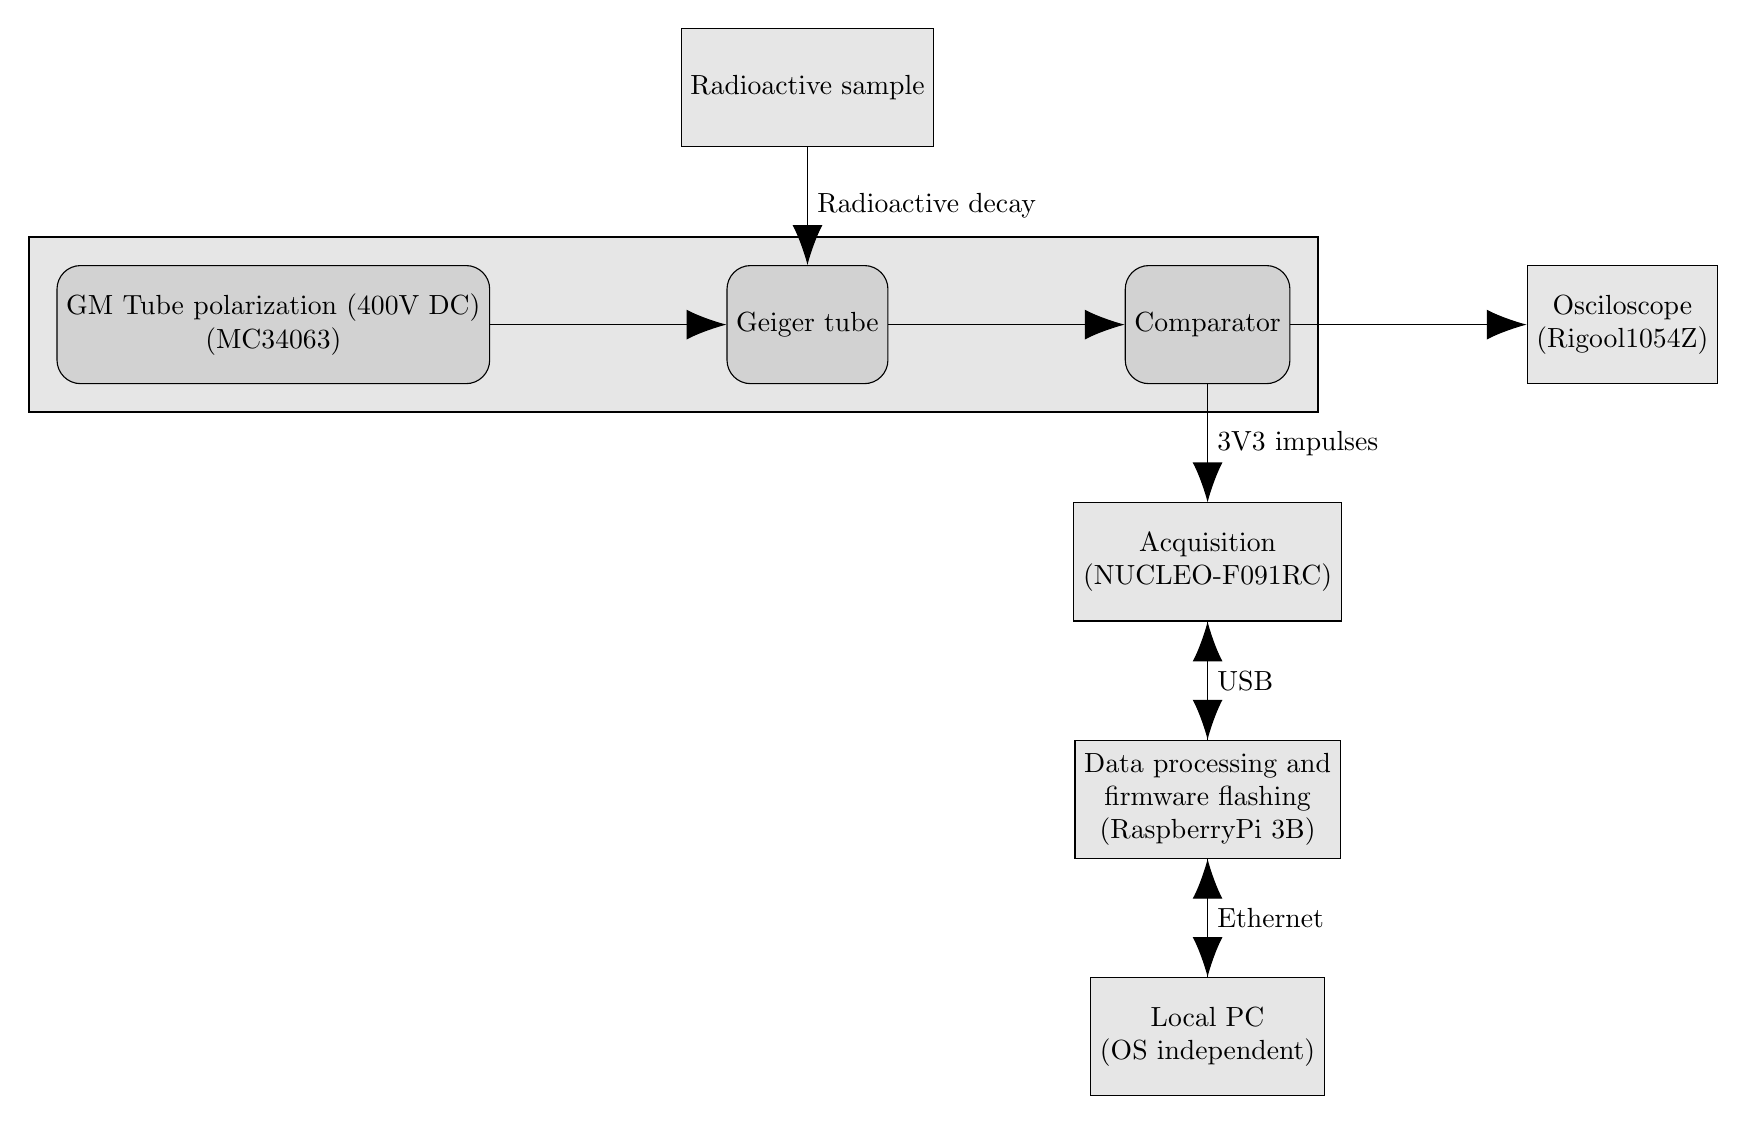
\begin{tikzpicture}[node distance=1.5cm and 3cm]
% Nodes
\pgfdeclarelayer{background}
\pgfsetlayers{background,main}

\node (gm_tube) [component] {Geiger tube};
\node (sample) [system, above=of gm_tube] {Radioactive sample};

\node (polarization) [component, left=of gm_tube] {GM Tube polarization (400V DC)\\ (MC34063)};
\node (comparator) [component, right=of gm_tube] {Comparator};

\node (osciloscope) [system, right=of comparator] {Osciloscope\\ (Rigool1054Z)};

\node (data_acquisition) [system, below=of comparator] {Acquisition\\ (NUCLEO-F091RC)};

\node (pi) [system, below=of data_acquisition] {Data processing and\\ firmware flashing\\ (RaspberryPi 3B)};
\node (pc) [system, below=of pi] {Local PC\\ (OS independent)};


\begin{pgfonlayer}{background}
\node[system ,  draw, thick,  inner xsep=1em, inner ysep=1em, fit=(gm_tube) (polarization) (comparator) ] {};
\end{pgfonlayer}

% Connectors
\begin{scope}[->]

\draw [-{Latex[scale=3.0]}] (sample) -- node[anchor=west, minimum width=.25cm, draw=none] {Radioactive decay} (gm_tube);
\draw [-{Latex[scale=3.0]}] (polarization) -- node[anchor=south, minimum width=.25cm, draw=none] {} (gm_tube);
\draw [-{Latex[scale=3.0]}] (gm_tube) -- node[anchor=south, minimum height=.25cm, draw=none] {} (comparator);
\draw [-{Latex[scale=3.0]}] (comparator) -- node[anchor=south, minimum height=.25cm, draw=none] {} (osciloscope);

\draw [-{Latex[scale=3.0]}] (comparator) -- node[anchor=west, minimum height=.25cm, draw=none] {3V3 impulses} (data_acquisition);
\draw [-{Latex[scale=3.0]}] (data_acquisition) -- node[anchor=west, minimum height=.25cm, draw=none] {USB} (pi);
\draw [-{Latex[scale=3.0]}] (pi) -- node[anchor=west, minimum height=.25cm, draw=none] {} (data_acquisition);

\draw [-{Latex[scale=3.0]}] (pi) -- node[anchor=west, minimum height=.25cm, draw=none] {Ethernet} (pc);
\draw [-{Latex[scale=3.0]}] (pc) -- node[anchor=west, minimum height=.25cm, draw=none] {} (pi);

\end{scope}

\end{tikzpicture}
\end{document}
